\documentclass[compress]{beamer}
\usepackage[latin1]{inputenc}
\usepackage{alltt}
\newdimen\topcrop
\topcrop=10cm  %alternatively 8cm if the pdf inclusions are in letter format
\newdimen\topcropBezier
\topcropBezier=19cm %alternatively 16cm if the inclusions are in letter format

\setbeamertemplate{footline}[frame number]
\title{Verifying a vertical cell decomposition algorithm}
\author{Yves Bertot\\
Thomas Portet}
\date{September 2025}
\mode<presentation>
\begin{document}

\maketitle
\begin{frame}
\frametitle{The overall picture}
\begin{itemize}
\item Find a path between obstacles
\item Obstacles are described by straight line segments
\item Decompose the working area into simple cells
\begin{itemize}
\item Each cell is safe
\item Each cell is convex
\item Each cell is non-empty
\end{itemize}
\item Moving from cells to neighbors is safe
\begin{itemize}
\item Cells have doors
\end{itemize}
\end{itemize}
\end{frame}
\begin{frame}
\frametitle{Example}
%trim parameters left bottom right top
\includegraphics[trim={0 0 0 \topcrop}, clip, width=\textwidth]{empty_spiral.pdf}
\end{frame}
\begin{frame}
\frametitle{Example : results}
%trim parameters left bottom right top
\includegraphics[trim={0 0 0 \topcrop}, clip, width=\textwidth]{cells_spiral3.pdf}
\end{frame}
\begin{frame}
\frametitle{Vertical cell decomposition}
\begin{itemize}
\item Use a vertical sweep line moving left to right
\item Stop each time one meets an edge tip (an event)
\item maintain a vertically ordered sequence of open cells
\begin{itemize}
\item close all open cells in contact with the event
\item open new cells forall edges starting at this event
\end{itemize}
\item Simplifying assumptions
\begin{itemize}
\item No vertical edges
\item Edges do not cross
\end{itemize}
\end{itemize}
\end{frame}
\begin{frame}
\frametitle{Intermediate position for vertical cell decomposition (1)}
%trim parameters left bottom right top
\includegraphics[trim={0 0 0 \topcrop}, clip, width=\textwidth]{partial_spiral.pdf}
\end{frame}
\begin{frame}
\frametitle{Intermediate position for vertical cell decomposition (2)}
%trim parameters left bottom right top
\includegraphics[trim={0 0 0 \topcrop}, clip, width=\textwidth]{partial_spiral2.pdf}
\end{frame}
\begin{frame}
\frametitle{Naive approach to cell generation}
\begin{itemize}
\item Maintain a sequence of ``open cells''
\item Compute cells in contact with the current event
\item Close cells in contact
\item Create new cells starting at the current event
\end{itemize}
\end{frame}
\begin{frame}
\frametitle{Illustration}
\begin{columns}
\begin{column}{0.3\textwidth}
%trim parameters left bottom right top
\includegraphics[trim={0 0 0 \topcrop}, clip, width=0.9\textwidth]{partial_spiral.pdf}
%trim parameters left bottom right top
\includegraphics[trim={0 0 0 \topcrop}, clip, width=0.9\textwidth]{partial_spiral2.pdf}
\end{column}
\begin{column}{0.7\textwidth}
\begin{itemize}
\item event in the middle of the pink area
\item open cells are pink, green, pink
\item contact cell: the pink cell
\item new closed cell: close the pink cell at the event,
obtain a dark red cell in the middle
\item new open cells: light blue and yellow
\end{itemize}
\end{column}
\end{columns}
\end{frame}
\begin{frame}
\frametitle{Difficulty with vertically aligned events}
\begin{itemize}
\item  Width of closed cells : horizontal distance between events
\begin{itemize}
\item Vertically aligned segments yield empty cells, if handled naively
\end{itemize}
\item Empty cells are a nuisance
\item Solution: special treatment
\begin{itemize}
\item Keep track of last open and closed cell
\item Update these cells instead of creating new ones
\end{itemize}
\end{itemize}
\end{frame}
\begin{frame}
\frametitle{Basic concepts}
\begin{itemize}
\item Edges: pairs of points with strict order on first coordinate
\item Points above, under, or on edges
\item Valid edges for a point
\item Edges below edges
\item Well-formed cells
\item Adjacent cells
\end{itemize}
\end{frame}
\begin{frame}
\frametitle{Above or under}
\begin{itemize}
\item Assume an edge with extremities \(l\) and \(r\) and an arbitrary point
\item \(\begin{array}{|ccc|}
1 & {\tt l}_x & {\tt l}_y\\
1 & {\tt r}_x & {\tt r}_y\\
1 & {\tt p}_x & {\tt p}_y\\
\end{array} > 0 \)
\quad if \(p\) is in the half plane above the edge.
\item edge \(g_1\) is below \(g_2\) if both extremities of \(g_2\) are above
\(g_1\) or both extremities of \(g_1\) are under \(g_2\)
\item Transitivity: if \(p_1\) and \(p_2\) are vertically aligned \(p_2\) is
above \(p_1\), if \(p_1\) is above an edge, then so is \(p_2\)
\item No transitivity for {\em edge below}
\end{itemize}
\end{frame}
\begin{frame}
\frametitle{Well-formed cells}
%trim parameters left bottom right top
\includegraphics[trim={0 19cm 0 4cm}, clip, width=\textwidth]{one_closed_cell.pdf}

\begin{itemize}
\item Open cells have no right points
\item Point sequences go from the high edge to the low edge
\item successive points on the point sequences describe safe doors
\item Open cells may be degenerate
\end{itemize}
\end{frame}
\begin{frame}
\frametitle{Cell assumptions}
\begin{itemize}
\item Vertical doors are safe passages between two cells
\item Moving from a left door  to a right door is safe
\begin{itemize}
\item and vice-versa
\end{itemize}
\item Moving from a left door to the cell center is safe
\begin{itemize}
\item similarly for a right-edge
\item moving from a left-side door to a left-side door is
safe by going through the cell center
\end{itemize}
\item These properties are guaranteed when cells are non-empty
\end{itemize}
\end{frame}
\begin{frame}
\frametitle{Non-vertically aligned events}
\begin{columns}
\begin{column}{0.3\textwidth}
%trim parameters left bottom right top
\framebox{\includegraphics[trim={5cm 20cm 6cm 0}, clip, width=0.9\textwidth]{simple_case1.pdf}}
\end{column}
\begin{column}{0.7\textwidth}
\begin{itemize}
\item The lower edge of the lower contact cell finishes further right
\item Also for the higher edge of the higher
\item All other contact cells have a pointy shape
\item The event may have outgoing edges
\item Before processing event \(e\), cells \(c_1\), \(c_2\), and \(c_3\) are
{\em open}
\item When processing event \(e\), these cells receive a right side at
the sweep line
\end{itemize}
\end{column}
\end{columns}
\end{frame}
\begin{frame}
\frametitle{Non-vertically aligned events: new open cells}
\begin{columns}
\begin{column}{0.3\textwidth}
%trim parameters left bottom right top
\framebox{
\includegraphics[trim={5cm 20cm 6cm 0}, clip, width=0.9\textwidth]{simple_case2.pdf}}
\end{column}
\begin{column}{0.7\textwidth}
\begin{itemize}
\item Two new open cells are created (in this case)
\item Their left side is at the sweep line
\end{itemize}
\end{column}
\end{columns}
\end{frame}
\begin{frame}
\frametitle{Non-vertically aligned events: next event}
\begin{columns}
\begin{column}{0.3\textwidth}
%trim parameters left bottom right top
\framebox{
\includegraphics[trim={5cm 20cm 6cm 0}, clip, width=0.9\textwidth]{simple_case3.pdf}}
\end{column}
\begin{column}{0.7\textwidth}
\begin{itemize}
\item Cell \(c_5\) is closed when processing \(e'\)
\item \(e'\) is safe for \(c_3\)
\end{itemize}
\end{column}
\end{columns}
\end{frame}
\begin{frame}
\frametitle{Vertically aligned events}
\begin{columns}
\begin{column}{0.3\textwidth}
%trim parameters left bottom right top
\framebox{\includegraphics[trim={5cm 20cm 6cm 0}, clip, width=0.9\textwidth]{bad_case1.pdf}}
\end{column}
\begin{column}{0.7\textwidth}
\begin{itemize}
\item Cell \(c_5\) is closed when processing \(e'\)
\item \(e'\) is safe for \(c_3\)
\end{itemize}
\end{column}
\end{columns}
\end{frame}
\end{document}



%%% Local Variables: 
%%% mode: latex
%%% TeX-master: t
%%% End: 
